\documentclass[12pt]{article}
\usepackage{graphicx}
\usepackage{hyperref}
\usepackage{amsmath}
\usepackage{amssymb}
\usepackage{siunitx}
\usepackage[numbers, square, sort&compress]{natbib}

\title{Chapter 11: Communicating Results from Molecular Docking}
\author{Elvis Martis}
\begin{document}
\maketitle


\section{Introduction}
Results obtained from molecular docking and related computational analyses are primarily intended to guide new experimental investigations or to provide a deeper interpretation of biological observations. Although experimental researchers may not specialise in computational methodologies, they possess strong expertise in the biological systems under study. Therefore, it is important to present computational findings clearly, avoiding unnecessary technical terminology that may obscure the key message. At the same time, it should be recognised that experimental scientists generally have a basic familiarity with computational approaches. When presenting results, each reported score or metric should be clearly explained, with particular emphasis on its potential physiological or biological relevance. Experimental researchers typically interpret new findings in relation to established reference data. Accordingly, in molecular docking studies, the scores obtained for newly designed molecules should be compared with those of known drugs or well-characterised reference compounds. Presenting the results within such a comparative framework provides appropriate context and makes the findings easier to interpret.

 This chapter aims to provide practical guidance on how to communicate docking results effectively to both expert and non-expert audiences in written manuscripts and presentations\cite{CH11_Berry2015,CH11_Forli2015,CH11_IsItReliable2018}. 


\section{Main outputs of molecular docking studies}

Most small-molecule docking workflows produce two kinds of output: predicted binding poses and numerical scores that approximate binding affinity\cite{CH11_Kitchen2004,CH11_Pagadala2017,CH11_AutoDockVina2010}.  A binding pose is a specific orientation and conformation of the ligand within the receptor binding site, typically represented as a three-dimensional atomic model\cite{CH11_Kitchen2004,CH11_Glide2004,CH11_cosconati2010}.  Docking scores are values computed by a scoring function using one of the following approaches or combination thereof, such as empirical, knowledge-based, or force field-based functions, into an approximate estimate of binding affinity\cite{CH11_Jain2006,CH11_EmpiricalScoring2018,CH11_Warren2006}. 

When communicating docking results, it is important to separate these two concepts for non-experts: the pose addresses \emph{where and how} the ligand binds, whereas the score addresses \emph{how favourable} that binding is predicted to be\cite{CH11_Kitchen2004,CH11_Forli2015,CH11_BindingAffinity2018}.  Experts will also appreciate an explicit statement of whether scores are being used only to rank-order compounds within a series, or whether any attempt is being made to interpret them as quantitative approximations of the binding free energy\cite{CH11_Warren2006,CH11_Plewczynski2011,CH11_BindingAffinity2018}. 

\section{Strengths and limitations}

Large benchmarking studies have shown that many docking programs can reproduce experimental binding modes to within 2 \r{A} root-mean-square deviation (RMSD) for a substantial fraction of protein--ligand complexes.\cite{CH11_Warren2006,CH11_Glide2004,CH11_Plewczynski2011}  In contrast, docking scores are much less reliable as predictors of absolute binding affinity, and their correlation with experimental data is modest\cite{CH11_Warren2006,CH11_EmpiricalScoring2018,CH11_BindingAffinity2018}. Furthermore, different docking engines and scoring functions often produce different best-ranked poses or compound lists, highlighting algorithmic dependence\cite{CH11_Plewczynski2011,CH11_ConsensusDocking2023,CH11_EmpiricalScoring2018}. Here, the algorithmic dependence encompasses both the conformational search algorithm and the scoring function used. Communicating these limitations explicitly is essential when addressing non-expert audiences, because there is a strong tendency to over-interpret small differences in docking scores as chemically meaningful\cite{CH11_BindingAffinity2018,CH11_IsItReliable2018,CH11_Berry2015}.  Studies examining self-docking and cross-docking have demonstrated that the top-scoring pose is not always the pose closest to the crystallographic reference. Particularly, in cross-docking exercise and difficult to tap binding sites, this limitation is largely magnified\cite{CH11_IsItReliable2018,CH11_Warren2006,CH11_cosconati2010}. Accordingly, docking results should be presented as a source of ranked hypotheses that require experimental validation. This should not be treated or assumed to be definitive proof of binding or relative potency\cite{CH11_Forli2015,CH11_Cheng2012,CH11_zhu2022}. 

\section{How to effectively communicate with different audiences?}

\subsection{Computational chemists and modellers}

For readers with a background in molecular modelling, the main communication challenge is to provide sufficient methodological and validation details so they can reproduce, critique, or extend the work.\cite{CH11_Berry2015,CH11_Kitchen2004,CH11_cosconati2010}  These experts will look for clear statements of software packages and versions, receptor structures and preparation protocols, sampling settings, scoring functions, and any post-processing or rescoring steps such as MM-GBSA or FEP\cite{CH11_Pagadala2017,CH11_Berry2015,CH11_EmpiricalScoring2018}. They will also expect documentation of validation steps such as re-docking, cross-docking, enrichment calculations, or retrospective virtual screening benchmarks\cite{CH11_Warren2006,CH11_Forli2015,CH11_Cheng2012}.  When writing for such an audience, figures can be more information rich, and can assume familiarity with jargon such as RMSD, enrichment factor, receiver operating characteristic (ROC) curves, or consensus scoring\cite{CH11_Forli2015,CH11_EmpiricalScoring2018,CH11_ConsensusDocking2023}.  Numerical tables can include both raw scores and derived metrics, such as $\Delta$ score within a series, Z-scores, or ranks, as long as the definitions are clearly stated\cite{CH11_EmpiricalScoring2018,CH11_Kitchen2004,CH11_Berry2015}.  Critical discussion of failed cases, for example, ligands with good scores but poor experimental activity, is particularly valuable\cite{CH11_BindingAffinity2018,CH11_IsItReliable2018,CH11_Plewczynski2011}. 

\subsection{Synthetic and medicinal chemists}

Synthetic and medicinal chemists are interested in how docking results support or challenge structure--activity relationships (SAR). They also keenly look to understand what appropriate modifications are suggested for lead optimisation programs\cite{CH11_Kitchen2004,CH11_Forli2015,CH11_cosconati2010}.  For this audience, qualitative descriptions of interactions, such as \emph{the added methoxy group forms a new hydrogen bond with a particular residue} or \emph{the bulky substituent clashes with a hydrophobic wall}, are often more informative than raw docking scores\cite{CH11_Berry2015,CH11_Glide2004,CH11_Kitchen2004}.  2D interaction diagrams, combined with a few representative 3D views, enable chemists to connect docking hypotheses with classical medicinal chemistry reasoning about hydrogen bonds, $\pi$--$\pi$ stacking, and steric effects\cite{CH11_Berry2015,CH11_Forli2015,CH11_zhu2022}.  

When discussing numerical scores with chemists, it is prudent to emphasise that only large changes in score within a congeneric series are likely to be meaningful and that scores from different programs cannot be compared directly\cite{CH11_BindingAffinity2018,CH11_EmpiricalScoring2018,CH11_Warren2006}.  Chemists also appreciate explicit statements about how docking guided compound selection, for example, whether compounds were filtered by score thresholds, visual inspection of poses, or predicted interactions with specific residues\cite{CH11_Forli2015,CH11_Cheng2012,CH11_zhu2022}.  Where possible, docking-derived hypotheses should be linked to experimentally measured structure--activity trends to reinforce or revise the current design strategy\cite{CH11_Cheng2012,CH11_cosconati2010,CH11_zhu2022}. 



\subsection{Biologists and pharmacologists}

Biologists and pharmacologists tend to focus on target biology, selectivity, and translation to functional assays and phenotypes\cite{CH11_zhu2022,CH11_Cheng2012,CH11_Forli2015}.  Docking results for this audience should be framed in terms of mechanistic hypotheses and testable predictions that connect molecular interactions with observed biological effects, such as altered potency, selectivity, or resistance profiles\cite{CH11_Kitchen2004,CH11_zhu2022,CH11_BindingAffinity2018}.  For example, a docking-based explanation of resistance might highlight how a mutation disrupts a key interaction or changes pocket shape, thereby rationalising a drop in potency\cite{CH11_Kitchen2004,CH11_Glide2004,CH11_Warren2006}.  Visuals for biologists should be simple, focusing on a limited number of key residues, annotated ligand features, and a clear orientation relative to known functional motifs, domains, or cofactors\cite{CH11_Berry2015,CH11_Forli2015,CH11_zhu2022}.  Avoid overwhelming this audience with details such as grid spacing, exhaustiveness, or technical details on scoring function; these can be relegated to methods sections or supplementary material\cite{CH11_Berry2015,CH11_Kitchen2004,CH11_cosconati2010}.  Instead, clearly discuss the confidence level in the docking model and how it integrates with other types of evidence, such as mutagenesis, kinetics, or structural biology\cite{CH11_Cheng2012,CH11_zhu2022,CH11_BindingAffinity2018}. 

\section{Communicating Docking in Research Articles}

\subsection{In the methods section}

A robust docking paper begins with a transparent and sufficiently detailed methods section\cite{CH11_Kitchen2004,CH11_Pagadala2017,CH11_Cheng2012}. Key elements include the receptor structure(s) used, with their Protein Data Bank identifiers, resolution, and any mutations, preparation steps (protonation, tautomers, missing loops), and how binding sites were identified and defined\cite{CH11_Berry2015,CH11_Pagadala2017,CH11_zhu2022}.  Ligand preparation should detail how protonation states, stereochemistry, and tautomers were enumerated, as well as the generation of 3D conformers\cite{CH11_Berry2015,CH11_Pagadala2017,CH11_Forli2015}. Docking protocol descriptions must name the software and version, specify search parameters, for example, number of poses, specific parameters depending on the docking program used, and identify the primary scoring function\cite{CH11_Pagadala2017,CH11_AutoDock4}.  If multiple docking engines or rescoring methods such as MM-GBSA were used, explain the workflow order and the criteria for advancing compounds between stages\cite{CH11_Berry2015,CH11_EmpiricalScoring2018,CH11_cosconati2010}. Finally, include a concise description of validation procedures, such as re-docking crystallographic ligands, cross-docking, and retrospective virtual screening benchmarks, along with the metrics used, such as RMSD, enrichment factor, and  area under the ROC curve\cite{CH11_Warren2006,CH11_Forli2015,CH11_ConsensusDocking2023}. 

\subsection{In the results and discussion section}

In this section, docking data should be presented in clear narratives that connect computational findings to chemical or biological questions\cite{CH11_Forli2015,CH11_Cheng2012,CH11_zhu2022}.  Instead of listing hundreds of scores, focus on representative compounds, key SAR patterns, and mechanistic explanations that are supported by both docking and experiment\cite{CH11_Kitchen2004,CH11_Forli2015,CH11_BindingAffinity2018}. For example, a chemical series may be discussed in terms of how added substituents extend into adjacent subpockets, alter hydrophobic complementarity, or introduce new interactions\cite{CH11_Glide2004,CH11_Kitchen2004,CH11_zhu2022}. Tables can summarise docking scores, ranks, and experimental potencies for a manageable subset of compounds, typically those that were synthesised or tested\cite{CH11_Berry2015,CH11_BindingAffinity2018,CH11_EmpiricalScoring2018}. Where full virtual screening campaigns are reported, aggregated metrics, such as enrichment factors at 1 \% and 5 \% of the ranked list, are often more meaningful than exhaustive hit lists\cite{CH11_Forli2015,CH11_Cheng2012,CH11_cosconati2010}.  Any discordances between docking predictions and experimental data should be acknowledged and, where possible, rationalised in terms of limitations of the scoring function, protein flexibility, or assay conditions\cite{CH11_Warren2006,CH11_BindingAffinity2018,CH11_zhu2022}.

\subsection{Figures: best practices for manuscripts}

High quality figures are central to effective communication of docking results\cite{CH11_Berry2015,CH11_Forli2015,CH11_zhu2022}. 
Common figure types include: 
\begin{itemize}
  \item 3D views of ligand poses in the binding pocket (\textbf{Figure \ref{fig:plots}A}), 
  \item 2D interaction diagrams(\textbf{Figure \ref{fig:plots}B}), 
  \item Overlays of multiple ligands or mutants, 
  \item Plots of enrichment or score--activity relationships\cite{CH11_Berry2015,CH11_Forli2015,CH11_EmpiricalScoring2018}. 
\end{itemize}
In all cases, legible labels, consistent colour schemes, for example, hydrogen bonds in one colour, hydrophobic regions in another, and simplified backgrounds help non-experts follow the key messages\cite{CH11_Berry2015,CH11_zhu2022,CH11_cosconati2010}. 

\begin{figure}[hbt!]
    \centering
    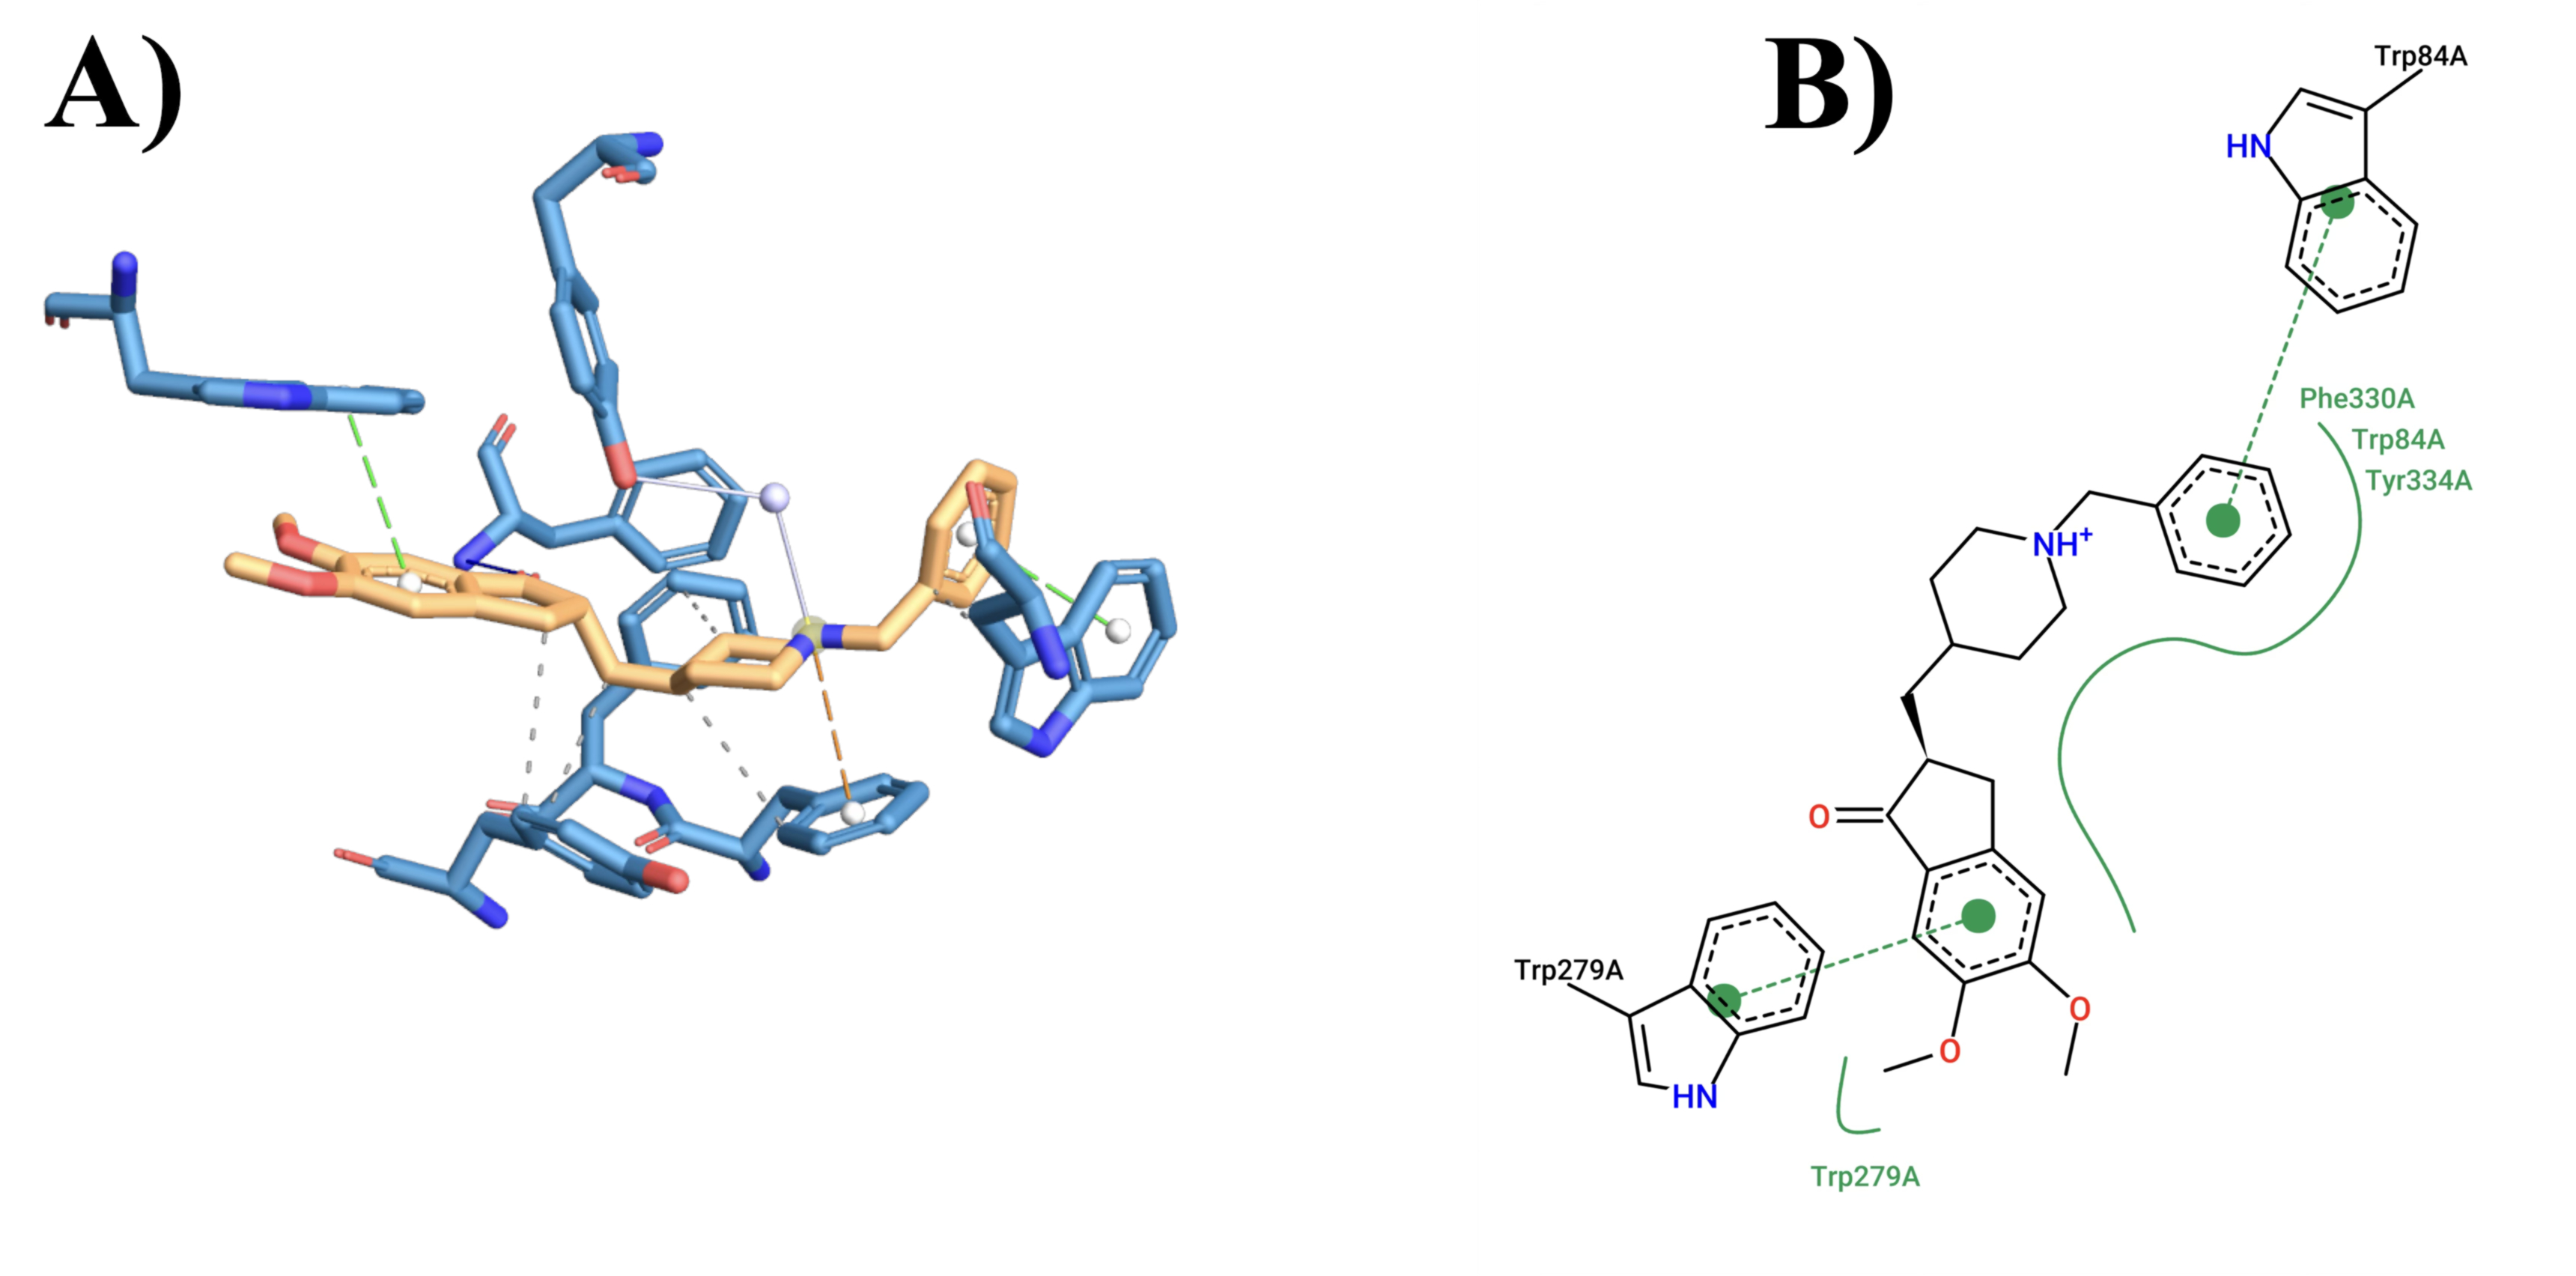
\includegraphics[width=1\textwidth]{3D_2D_plots.jpg}
    \caption{An illustration of protein-ligand interaction of Donepezil bound to acetylcholinesterase (PDB id: 1EVE). \textbf{A.} 3D interaction diagram where donepezil is shown in orange tube, and \textbf{B.} 2D interaction plot.}
\label{fig:plots}
\end{figure}

For 3D pose figures, choose viewpoints that clearly reveal interactions of interest and avoid occlusion; show only the relevant region of the protein to reduce clutter\cite{CH11_Berry2015,CH11_Glide2004,CH11_Forli2015}.  2D diagrams generated by widely used toolkits can be annotated manually to emphasise which interactions are considered critical for binding or selectivity\cite{CH11_Berry2015,CH11_Cheng2012,CH11_zhu2022}.  When presenting score versus activity plots, include trend lines and indicate the typical uncertainty or expected scatter so that readers do not over-interpret apparently tight correlations\cite{CH11_BindingAffinity2018,CH11_EmpiricalScoring2018,CH11_Warren2006}. 


\subsection{Discussing uncertainty and avoiding over-claiming}

A recurring weakness in docking papers is overconfident language about predictions. One should avoid implying that docking alone proves binding, selectivity, or mechanism. Instead, docking should be framed as a source of hypotheses to be tested experimentally\cite{CH11_Cheng2012}.  Phrases such as \emph{consistent with}, \emph{suggests that}, or \emph{is compatible with} better reflect the inferential nature of docking results\cite{CH11_IsItReliable2018}.  It is also important to state explicitly what docking cannot address in a given study, for example, induced-fit effects, allosteric conformational changes, water-mediated networks, or entropic contributions that are not well captured by the scoring function. Studies focused on binding affinity should acknowledge that more rigorous methods, such as MM-GBSA, MM-PBSA, or free energy calculations, are required for robust quantitative predictions. Despite this system dependence, uncertainty remains\cite{CH11_EmpiricalScoring2018,CH11_Berry2015}.

\section{Communicating Docking in Presentations}

\subsection{Structuring}

In live talks and seminars, attention spans are limited, so docking results must be tightly integrated into a broader scientific story. An effective structure is to begin with the biological or chemical question, then outline why docking was the appropriate tool, briefly describe the key aspects of the protocol, and finally present a small number of high-impact findings. This approach helps non-experts understand where docking fits into the overall project rather than perceiving it as an isolated computational exercise. When time is short, details such as grid sizes, exact scoring functions, or all validation metrics can be relegated to backup slides or supplementary materials. Instead, focus the main presentation on how docking guided compound prioritisation, explained unexpected SAR, or generated mechanistic hypotheses that were subsequently tested. Explicitly connecting docking predictions to experimental decisions, such as which analogues were synthesised next, makes the value of the methodology tangible to non-modellers\cite{CH11_Berry2015,CH11_Forli2015,CH11_Pagadala2017}.

\subsection{Designing visuals}

Effective docking figures for presentations are even simpler than those for manuscripts, because audiences must parse them in seconds. Use large fonts, high contrast colours, and minimal text; annotate only the most critical residues and ligand features. It is often helpful to start with a cartoon of the protein domain architecture or overall fold before zooming into the binding pocket, to provide biologists with a familiar context. Avoid showing more than two or three overlaid poses in a single 3D figure, as excessive overlap can confuse even experts. When comparing wild-type and mutant proteins or different chemotypes, separate slides with side-by-side panels often work better than dense multi-overlays.
Score tables should be limited to a few representative compounds, ideally with colour-coding or icons to indicate whether each was an experimentally confirmed hit, a borderline case, or a false positive.

\subsection{Handling questions and scepticism}

The reliability of docking is a topic of ongoing debate; presenters should anticipate questions about validation, false positives, and false negatives\cite{CH11_BindingAffinity2018,CH11_Plewczynski2011}.  Having one or two backup slides summarising re-docking RMSDs, enrichment metrics, or retrospective benchmarks can be very helpful. If docking failed for certain chemotypes or targets, acknowledging these limitations and offering plausible reasons, such as highly flexible binding sites or covalent mechanisms.  

When biologists or chemists challenge specific predictions, they emphasise that docking was used as a heuristic to prioritise experiments rather than as a replacement for empirical testing\cite{CH11_Forli2015,CH11_Cheng2012,CH11_zhu2022}. Conversely, when docking successfully rationalises SAR or guides a successful hit discovery, avoid overstating its general applicability beyond the studied system. These balanced statements and interpretations reinforce the idea that docking is powerful when used judiciously to complement, rather than replace, experiments\cite{CH11_Forli2015,CH11_zhu2022,CH11_cosconati2010}.

\section{Special Topics and Advanced Cases}

\subsection{Consensus docking and rescoring}

One way to improve confidence in docking predictions is to combine results from multiple docking engines or scoring functions, an approach known as consensus docking or consensus scoring. Analyses of large benchmark sets have shown that consensus strategies can improve enrichment and pose prediction at the cost of increased computational effort. When reporting consensus docking, one should clearly describe how the consensus was constructed, for example, majority vote on actives, averaged ranks, or intersection of top-ranked subsets\cite{CH11_ConsensusDocking2023,CH11_Plewczynski2011}. Similarly, re-scoring docked poses with more physics-based methods such as MM-GBSA/PBSA or LIE can improve the ranking of actives within a focused set, although performance remains target-dependent\cite{CH11_Berry2015,CH11_cosconati2010}.  Communicating these advanced methods to non-experts requires careful simplification, for instance, describing MM-GBSA as a \emph{more detailed energy calculation} that refines the coarse docking scores. Where possible, present side-by-side comparisons showing how rescoring improved the correlation with experimental data or enriched actives in the top-ranked subset\cite{CH11_zhu2022}. 

\subsection{Covalent docking, induced-fit, and flexibility}

Standard docking tools typically assume a rigid receptor and non-covalent binding, which is an important caveat when communicating results on covalent inhibitors or highly flexible targets. Specialised protocols and software exist for covalent and induced-fit docking; however, they introduce additional assumptions and parameters that must be described transparently\cite{CH11_AutoDock4,CH11_Glide2004,CH11_zhu2022}. When presenting such studies, clearly differentiate between non-covalent pre-orientation, covalent bond formation, and any subsequent relaxation of the protein--ligand complex\cite{CH11_AutoDock4,CH11_Kitchen2004}.  For systems where protein flexibility is critical, ensemble docking or integration with molecular dynamics (MD) simulations can provide more realistic pictures of binding. Communicating these approaches effectively often involves showing how multiple receptor conformations contribute to binding, for example, via cluster representatives or occupancy maps. Non-experts generally benefit from high-level explanations, like \emph{we used several snapshots to capture different shapes of the pocket}, rather than algorithmic details.

\section{Practical Recommendations}

\subsection{For manuscripts}

For manuscripts reporting docking, the following checklist can help ensure clear and responsible communication:

\begin{itemize}
  \item Clearly state the biological or chemical question that docking is addressing, and why docking is appropriate for this question.
  \item Provide sufficient methodological detail on receptor and ligand preparation, software, parameters, and scoring to ensure reproducibility.
  \item Describe validation procedures, such as re-docking, cross-docking, enrichment, and report standard metrics such as RMSD and enrichment factors.
  \item Use figures and tables that emphasise representative poses, key interactions, and SAR, rather than exhaustive score lists.
  \item Explicitly acknowledge the known limitations of docking and the uncertainty associated with scores and poses.
  \item Integrate docking results with experimental data to build coherent mechanistic narratives and prioritise hypotheses.
\end{itemize}

\subsection{For presentations}

For presentations to mixed audiences, a complementary checklist is useful:

\begin{itemize}
  \item Begin with the biological or medicinal chemistry problem and only then introduce docking as a tool.
  \item Limit the number of docking figures and ensure each has a single clear message.
  \item Avoid technical jargon unless the audience is predominantly computational and, even then, define specialised terms briefly.
  \item Highlight how docking influenced experimental design, compound selection, or mechanistic interpretation.
  \item Prepare backup slides with methodological details and validation metrics for expert questions.
  \item Use cautious language about predictive accuracy and always link predictions to plans for experimental validation.
\end{itemize}

\bibliographystyle{unsrtnat}
\bibliography{chapter11}


\end{document}